%%%%%%%%%%%%%%%%%%%%%%%%%%%%%%%%%%%%%%%%%
% Beamer Presentation
% LaTeX Template
% Version 1.0 (10/11/12)
%
% This template has been downloaded from:
% http://www.LaTeXTemplates.com
%
% License:
% CC BY-NC-SA 3.0 (http://creativecommons.org/licenses/by-nc-sa/3.0/)
%
%%%%%%%%%%%%%%%%%%%%%%%%%%%%%%%%%%%%%%%%%

%----------------------------------------------------------------------------------------
%	PACKAGES AND THEMES
%----------------------------------------------------------------------------------------

\documentclass{beamer}

\mode<presentation> {

% The Beamer class comes with a number of default slide themes
% which change the colors and layouts of slides. Below this is a list
% of all the themes, uncomment each in turn to see what they look like.

%\usetheme{default}
%\usetheme{AnnArbor}
%\usetheme{Antibes}
%\usetheme{Bergen}
%\usetheme{Berkeley}
%\usetheme{Berlin}
%\usetheme{Boadilla}
%\usetheme{CambridgeUS}
%\usetheme{Copenhagen}
%\usetheme{Darmstadt}
%\usetheme{Dresden}
%\usetheme{Frankfurt}
%\usetheme{Goettingen}
%\usetheme{Hannover}
%\usetheme{Ilmenau}
%\usetheme{JuanLesPins}
%\usetheme{Luebeck}
\usetheme{Madrid}
%\usetheme{Malmoe}
%\usetheme{Marburg}
%\usetheme{Montpellier}
%\usetheme{PaloAlto}
%\usetheme{Pittsburgh}
%\usetheme{Rochester}
%\usetheme{Singapore}
%\usetheme{Szeged}
%\usetheme{Warsaw}

% As well as themes, the Beamer class has a number of color themes
% for any slide theme. Uncomment each of these in turn to see how it
% changes the colors of your current slide theme.

%\usecolortheme{albatross}
%\usecolortheme{beaver}
%\usecolortheme{beetle}
%\usecolortheme{crane}
%\usecolortheme{dolphin}
%\usecolortheme{dove}
%\usecolortheme{fly}
%\usecolortheme{lily}
%\usecolortheme{orchid}
%\usecolortheme{rose}
%\usecolortheme{seagull}
%\usecolortheme{seahorse}
%\usecolortheme{whale}
%\usecolortheme{wolverine}

%\setbeamertemplate{footline} % To remove the footer line in all slides uncomment this line
%\setbeamertemplate{footline}[page number] % To replace the footer line in all slides with a simple slide count uncomment this line

%\setbeamertemplate{navigation symbols}{} % To remove the navigation symbols from the bottom of all slides uncomment this line
}

\usepackage{graphicx} % Allows including images
\usepackage{booktabs} % Allows the use of \toprule, \midrule and \bottomrule in tables
\usepackage{framed}
%----------------------------------------------------------------------------------------
%	TITLE PAGE
%----------------------------------------------------------------------------------------

\title[Introduzione]{Creational Patterns} % The short title appears at the bottom of every slide, the full title is only on the title page

\author{Claudio Menghi,  Srdan Krstic} % Your name
\institute[Deepse group] % Your institution as it will appear on the bottom of every slide, may be shorthand to save space
{
Politecnico di Milano \\ % Your institution for the title page
\medskip
\textit{menghi@elet.polimi.it,  srdan.krstic@polimi.it} % Your email address
}
\date{\today} % Date, can be changed to a custom date

\begin{document}


\begin{frame}
\titlepage % Print the title page as the first slide
\end{frame}


\begin{frame}
\frametitle{Overview} % Table of contents slide, comment this block out to remove it
\tableofcontents % Throughout your presentation, if you choose to use \section{} and \subsection{} commands, these will automatically be printed on this slide as an overview of your presentation
\end{frame}


\section{Design Principles}



\begin{frame}
\frametitle{Design Principles}
Open Close Principle
\begin{framed}
Le entit\`a del software (le classi, i moduli e le funzioni) devono essere \emph{aperte all'estensione} e \emph{chiuse alle modifiche}\\
\end{framed}
\end{frame}

\begin{frame}
\frametitle{Design Principles}
Dependency Inversion Principle
\begin{framed}
I moduli di alto livello non devono dipendere direttamente dai moduli di basso livello. Entrambi devono dipendere da delle astrazioni.
\end{framed}
Quando delle classi di alto livello devono accedere a delle risorse di basso livello (disco I/O etc..) \`e conveniente
\end{frame}


\begin{frame}
\frametitle{Design Principles}
Single Responsibility Principle
\begin{framed}
A class should have only one reason to change.
\end{framed}
\end{frame}

\begin{frame}
\frametitle{Design Principles}
Liskov's Substitution Principle
\begin{framed}
Derived types must be completely substitutable for their base types.
\end{framed}
\end{frame}


%----------------------------------------------------------------------------------------
%	PRESENTATION SLIDES
%----------------------------------------------------------------------------------------

\section{Pattern}

\begin{frame}
\frametitle{Design Patterns}

\begin{itemize}
\item Pattern	creazionali: riguardano	il	processo	di	creazione	di	oggetti	
\item Pattern	strutturali	: hanno	a	che	fare	con	la	composizione	di	classi	ed	 oggetti
\item Pattern	comportamentali: Si	occupano	di	come	interagiscono	gli	oggetti	e	distribuiscono	fra	loro	le	responsabilit\`a
\end{itemize}


\end{frame}

\subsection{Creational Pattern}

\begin{frame}
\frametitle{Creational Patterns}
\begin{itemize}
\item Abstract	Factory:	Creates	an	instance	of	several	families	of	classes	
\item Factory	Method:	Creates	an	instance	of	several	derived	classes
\item Singleton:	A	class	of	which	only	a	single	instance	can	exist	
\item Prototype:	A	fully	initialized	instance	to	be	copied	or	cloned	
\item Builder:	Separates	object	construction	from	its	 representation	
\end{itemize}
\end{frame}

\begin{frame}
\frametitle{Factory method}
\begin{figure}
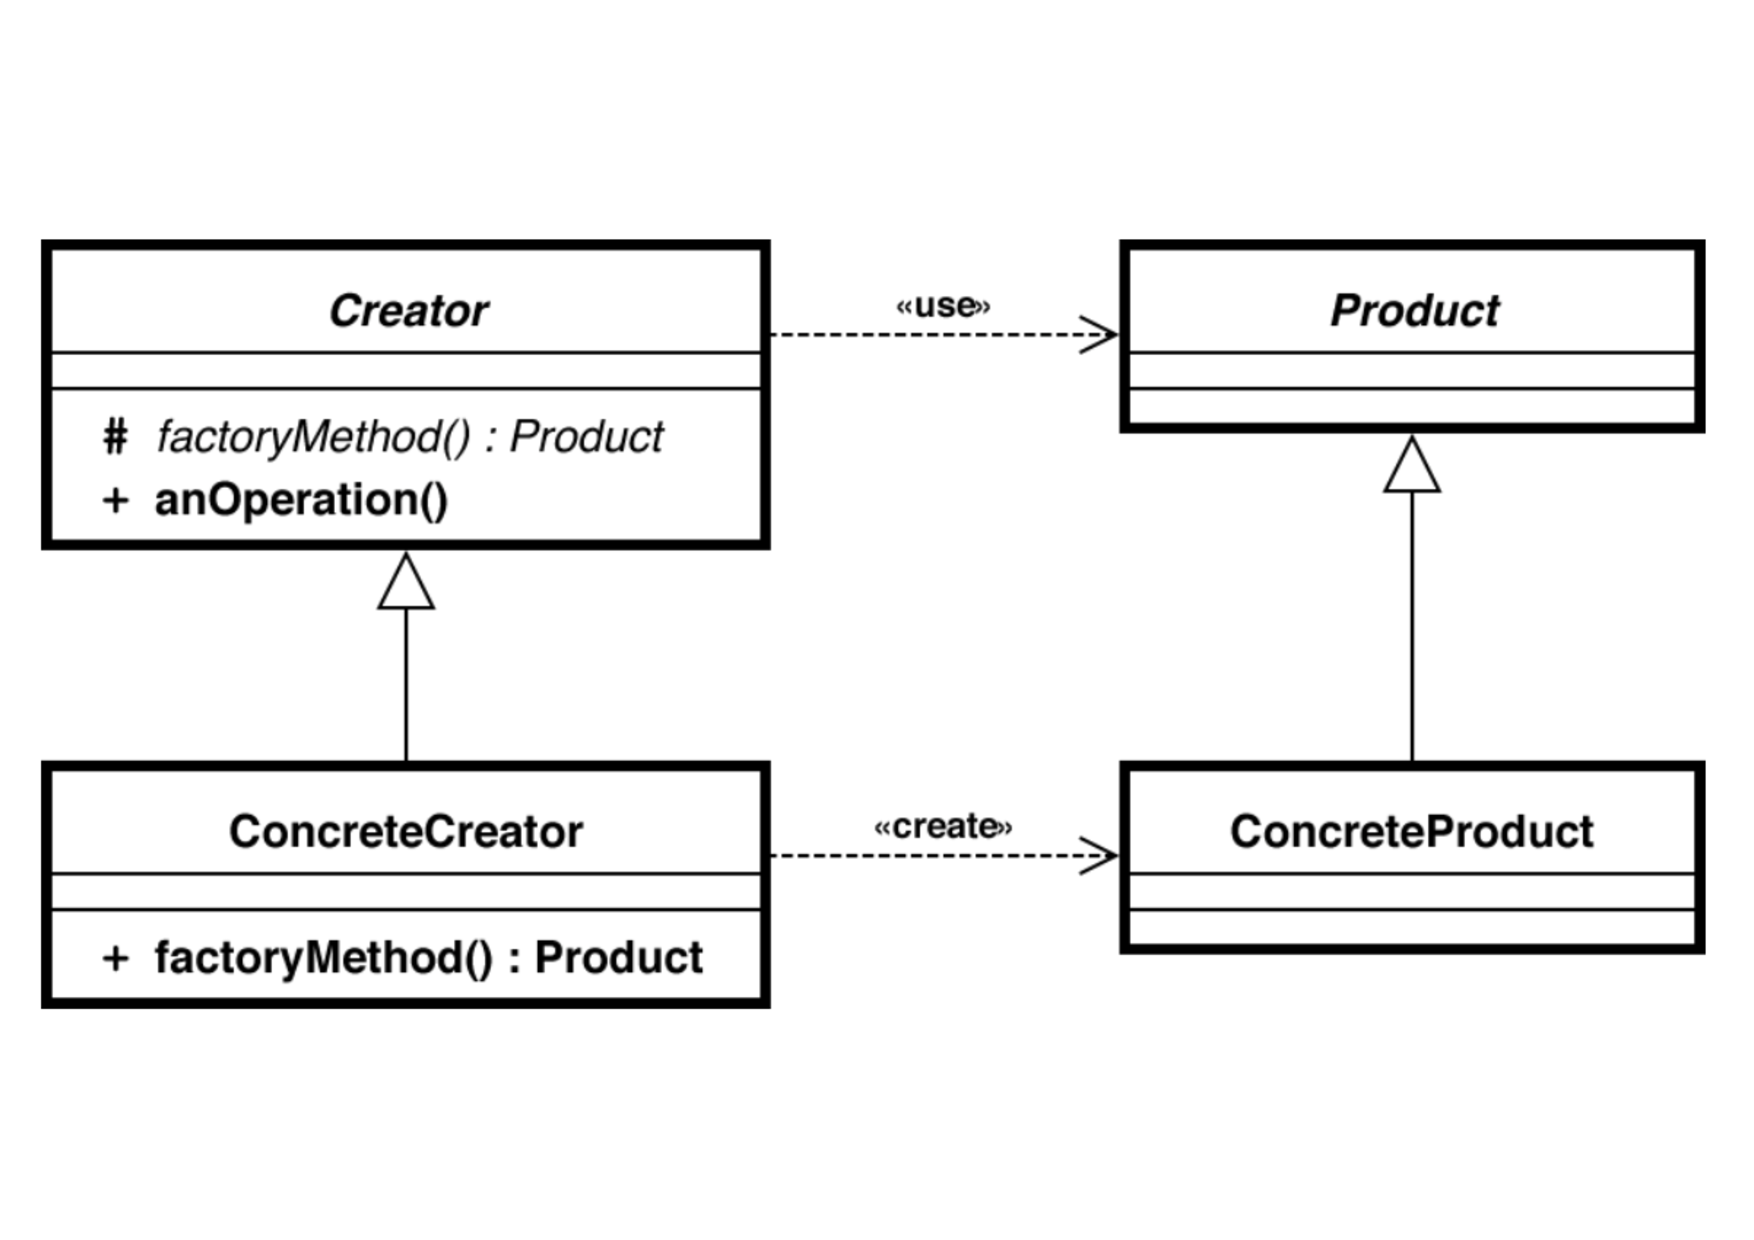
\includegraphics[width=0.8\textwidth]{Img/FactoryMethodDescription.pdf}
\end{figure}
\end{frame}

\begin{frame}
\frametitle{Abstract factory}
\begin{figure}
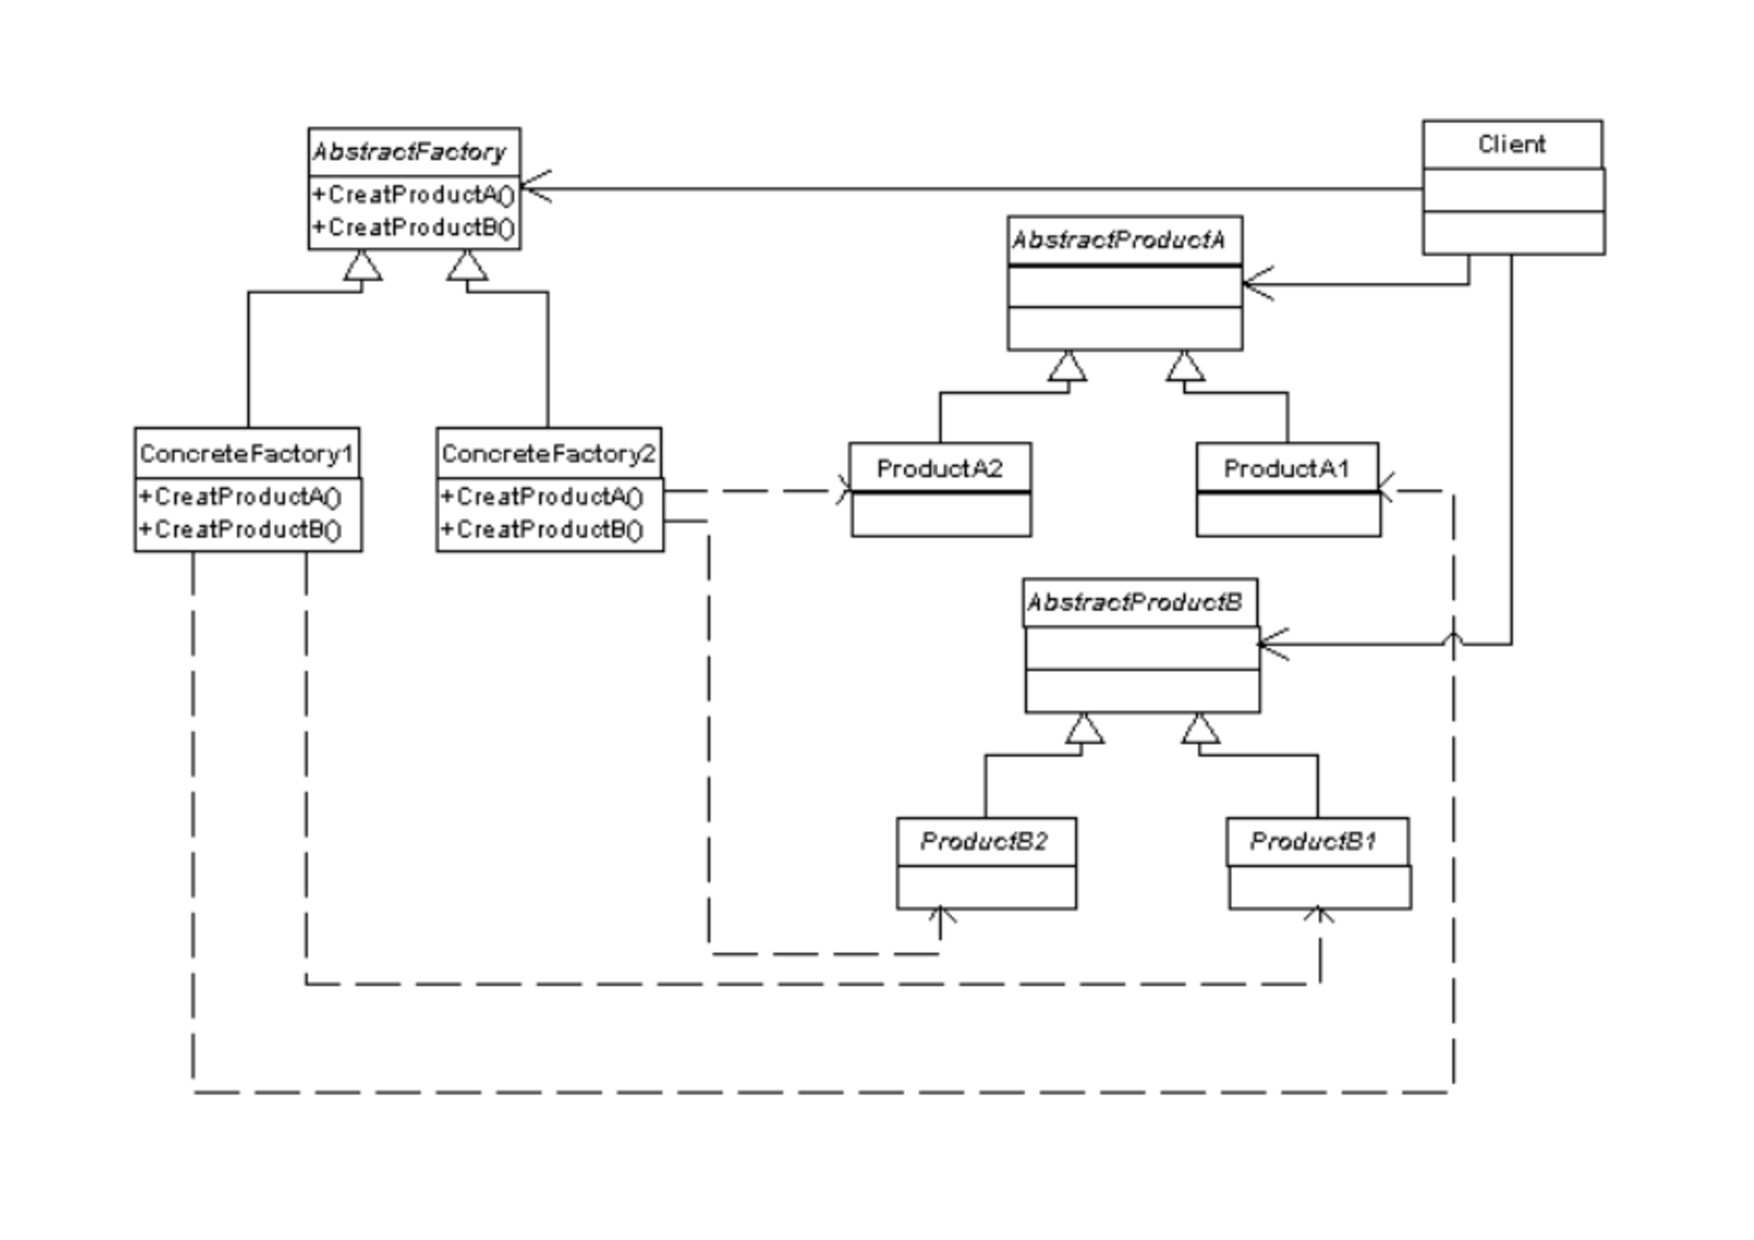
\includegraphics[width=1\textwidth]{Img/AbstractFactoryDescription.pdf}
\end{figure}
\end{frame}

\begin{frame}
\frametitle{Singleton}
\begin{figure}
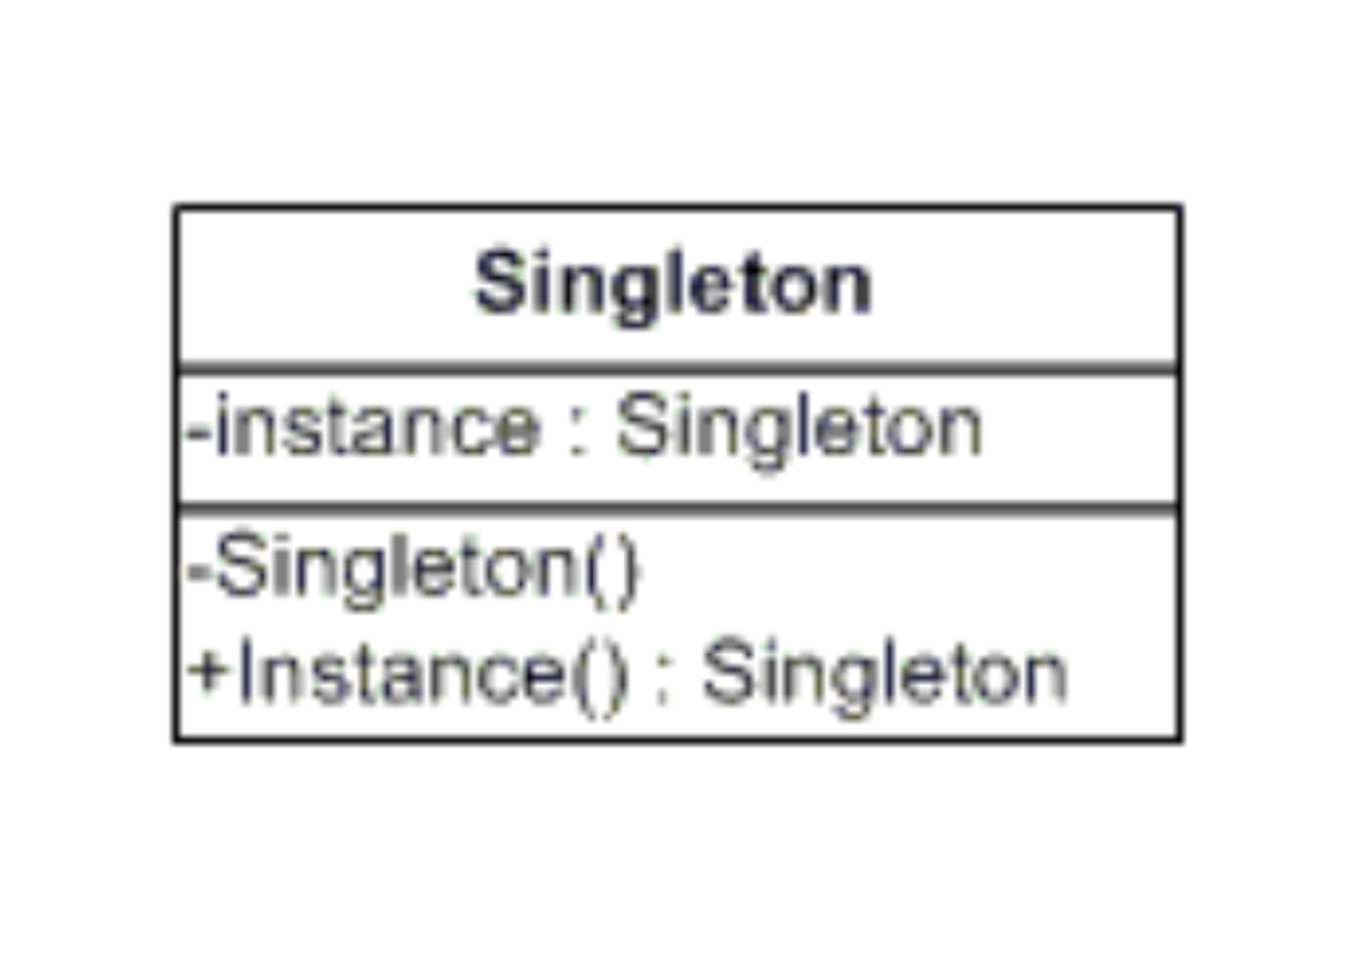
\includegraphics[width=0.5\textwidth]{Img/Singleton.pdf}
\end{figure}
\end{frame}

\section{Esercizi}

\subsection{Esercizio 1}

\begin{frame}
\frametitle{Esercizio 1}
\begin{framed}
Esercizio 2: implementare un gioco contenente un labirinto. Il labirinto deve essere composto da locali, porte e muri. Ogni locale ha quattro pareti, nord sud est ovest che possono essere occupati da un muro o da una porta. Deve essere possibile anche creare un tipo di labirinto bombato, dove ogni 3 porte viene creata una porta bombata.
\end{framed}
\end{frame}

\subsection{Esercizio 2}
\begin{frame}
\frametitle{Esercizio 2}
\begin{framed}
Esercizio 1: implementare una classe che rappresenta il sacco di Babbo Natale. Il sacco di Babbo Natale non contiene elementi, ma Babbo Natale pu\`o estrarre dei giocattoli che possono essere randomicamente  Pinguini, Draghetti o Dinosauri (con probabilit\`a 1/3 ad ogni estrazione, tranne quando gli elementi di un tipo sono finiti). Al pi\`u Babbo Natale pu\`o estrarre 20 elementi per ogni tipo. Ogni giocattolo ha un numero seriale (generato in maniera incrementale).
\end{framed}
\end{frame}



\subsection{Esercizio 3}
\begin{frame}
\frametitle{Esercizio 3}
\begin{framed}
Esercizio 3: Deve essere possibile creare labirinti di vario tipo. Per esempio un labirinto incantato deve contenere dei locali incantati, delle porte parlanti etc. Un labirinto esterno contiene delle porte in sasso (per aprire tale porte \`e necessario avere una determinata energia).
\end{framed}
\end{frame}


\subsection{Esercizio 4}
\begin{frame}
\frametitle{Esercizio 4}
\begin{framed}
Esercizio 4: Non ha senso creare istanze differenti del \texttt{LabirintoMagicoCreator} e del \texttt{LabirintoEsternoCreator}. Per ottenere vari labirinti verr\`a chiamato diverse volte il metodo \texttt{createLabirinto} che ritorner\`a istanze diverse della classe \texttt{Labirinto}.
\end{framed}
\end{frame}




%----------------------------------------------------------------------------------------

\end{document} 